% Chapter 2

\chapter{Basics} % Main chapter title

\label{Chapter2} % For referencing the chapter elsewhere, use \ref{Chapter2} 

This chapter introduces some preliminaries for this thesis. It explains the process of modern software development with highlights to keywords like \emph{Software release lifecycle} and \emph{Product release lifecycle} and is intended to answer the following question.

\vspace{0.5cm}
\noindent Question 1: What is Software Integration and Software Delivery ?
\vspace{0.5cm}


\noindent The primary section of this chapter presents the basic concept of integration and delivery and outlines a method to automate the process. The second part of this chapter summarize the key aspects of \ac{SCM} and Release Management, and lay its importance in a comprehensive manner (see Section~\ref{section:Softwareconfigurationmanagement}). Furthermore, it explains the key terminologies used in Software Versioning. The last part of the chapter (Section~\ref{section:embeddedlinux}) outlines the basics of Embedded Linux distribution with reference to components of the Yocto project and the \ac{OE} build system. 



%----------------------------------------------------------------------------------------

\section{Software Integration}\label{section:SoftwareIntegration}
\emph{Software Integration} is defined by the process of bringing software packages and applications to work closely with one another and extending its functionalities to the fullest potential without hindering its quality. It has multiple use cases and advantageous in terms of better software productivity and offers better quality. The past decade has witnessed a surge in software development and some significant changes in terms of integration and deployment of software packages. In today’s world, the culture of DevOps is integrated into projects which brings in automation to the stages of software build and testing and introducing key terms like \emph{automated release management}. This ultimately improves the product and software release lifecycle and provide a better software quality.    

%----------------------------------------------------------------------------------------
%\subsection{Advantages} \label{section:applicationsoftwareintegration}
\vspace{0.5cm}
\noindent \textbf{Advantages}
\vspace{0.5cm}

\noindent The software integration process includes multiple stages like code build, compilation, testing, deployment, operations, among others. The long process of software integration have been an area of key concern in software engineering~\parencite{vasilescu2015quality}, but it was majorly addressed by the introduction of \ac{CI} \ac{CD} (see figure \ref{fig:Continuous Integration approach}). The approach is further boosted by the introduction of the \ac{CI} server and verified by an automated build pipeline which takes care of the necessary stages of integration. Automated servers like \emph{CruiseControl}, \emph{Jenkins}, among others can further streamlined the \ac{SDLC} and can prevent the “it works on my machine” syndrome  before the code hits production~\parencite{6802994}. The above stated advantages is also practically confirmed in the preliminary thesis work mentioned in chapter \ref{Chapter3}, where the in-focus software package is continuously integrated with the help of a build pipeline (see Section~\ref{section:ImplementationOutline}).


In figure \ref{fig:Continuous Integration approach}, the basic model of the {\ac{CI}} process is outlined with the help of the Jenkins automated server. It takes advantage of a version control system tool, shared among several developers to store the project source code in a shared repository. Now, with every change committed to the source code, configurations or other data, a new instance of the pipeline gets triggered. After a successful build, the subsequent steps of delivery and deployment are executed.  

\vspace{0.5cm}
\begin{figure}[H]
\centering{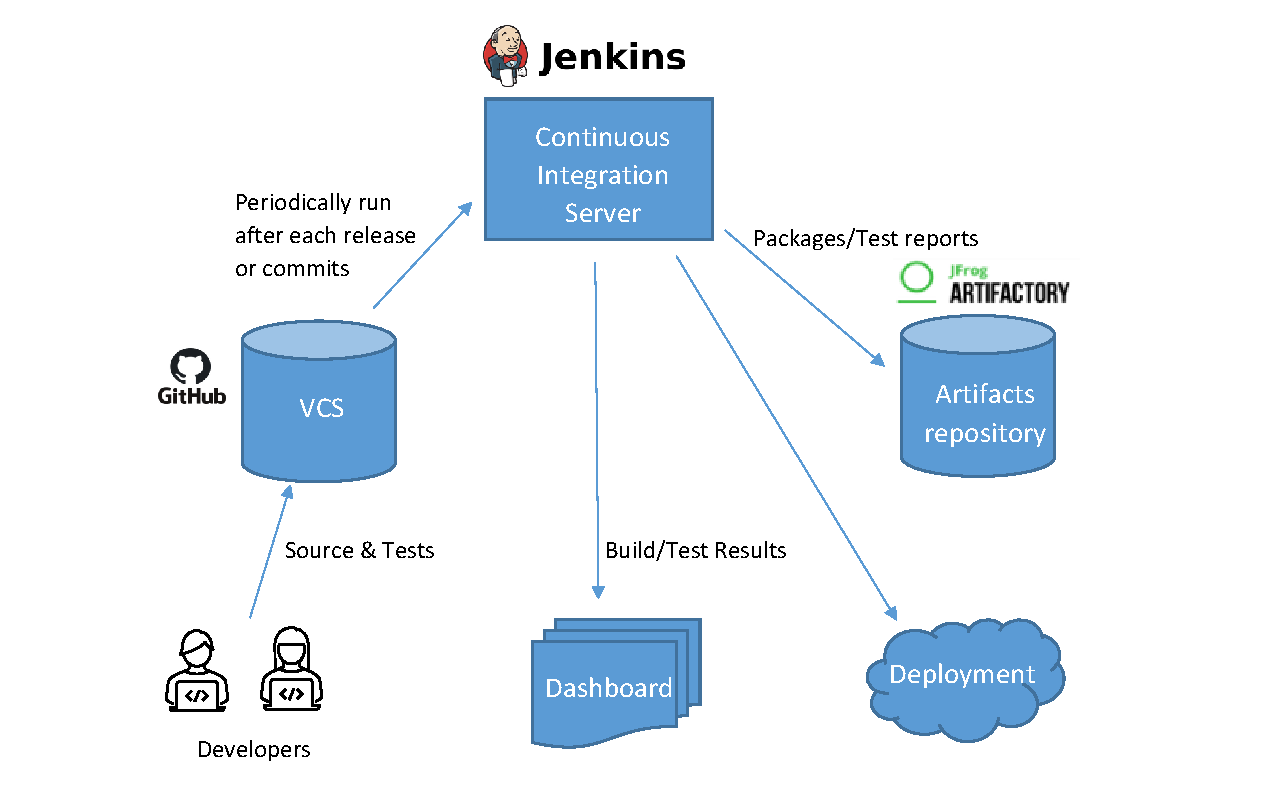
\includegraphics[width=1\textwidth]{figures/SoftwareIntegration.pdf} }%
\caption[Continuous Integration approach]{An integration build process\footnotemark}
\label{fig:Continuous Integration approach}
\end{figure}
\vspace{0.5cm}

\footnotetext{Cited from \parencite[p-4]{ant}.}
%reference image "A typical software process using a \ac{CI} approach." taken 
%----------------------------------------------------------------------------------------
\section{Software Delivery}\label{section:SoftwareDelivery}

The term Software Delivery in IT defines a complete phase where software components get all the updates, fixes, features delivered to customer or clients securely and hassle free. It might be confusing for the readers to contemplate which exact software components are being delivered. In context to this thesis work, software components includes the applications or product images, developed within the department. To understand this concept of Software Delivery in a better way, consider the process of software development within Bosch. The initial phase involves requirement analysis and development. Once the development phase is completed, the software components go through quality assurance test and operations before the actual delivery to the customer. The approach of testing software applications or components is vital to the software quality but if maintained in a traditional way, the delivery takes time and also involves manual effort. Often the delivery time of these applications or products gets delayed. So, almost companies over the world including BOSCH Group, have welcomed the idea of modern delivery technique. In other words, it can also be called as \emph{Continuous Delivery and Deployment}. In a precise way, the term Continuous Deployment means that each commit to the repository is automatically released to production. With Continuous Delivery, each commit ends up with a release candidate, allowing production release to be done manually~\parencite{leszko2017continuous}.

The next few sections will throw light on the traditional delivery approach and its shortcomings and why the modern software delivery technique have welcomed the idea of continuous delivery and deployment of products and software applications. 


\subsection{Traditional delivery process}

Software applications and products have release cycle defined within projects which starts off with the requirement stage, followed by development, quality strategy and lastly operations. This delivery process takes considerable amount of time due to the involvement of manual QA (\ac{UAT}, Integration testing and various other non-functional testing). An error detected by the tester at QA stage has to be passed on to the development stage again, to get it fixed by the developer and then roll back to the QA stage to test the same features. This process have multiple shortcomings as it lacks automation and also the delivery process becomes comparatively slow and requires effective communication between the teams.

\subsection{Modern delivery process}

Modern delivery process is all about fulfilling the shortcomings of traditional approaches of software delivery by bringing in automation into projects and introducing \emph{automated delivery pipeline} or \emph{continuous delivery}~\parencite{leszko2017continuous}. It simply means that with each bug fixes or code changes, the delivery timeline or the application release cycle or the product release cycle doesn't gets hampered.The most accurate definition of continuous delivery is stated by Jez Humble and reads as follows~\parencite{leszko2017continuous}:
\vspace{0.5cm}


\enquote{\emph{Continuous Delivery is the ability to get changes of all types-including new features, configuration changes, bug fixes, and experiments-into production, or into the hands of users, safely and quickly in a sustainable way.}}


\vspace{0.5cm} 

With continuous delivery, the software package or the application is deployed continuously into artifact repository against a development release version or to production.

For example, the DevOps (indicated by the orange block in figure \ref{fig:DevOps model}) model is highly valued in the industry. It combines the entire operations and QA tasks into an automated software delivery pipeline that can be handled by the development team itself~\parencite{leszko2017continuous}. DevOps platform like Jenkins, GitHub and technologies like containers and Kubernetes offers flexibility according to the organizational needs. The overall continuous delivery approach reduces lot of time and error-prone manual effort by bringing in automation into the delivery process of software or product.

%----------------------------------------------------------------------------------------
\vspace{0.5cm}
\begin{figure}[H]
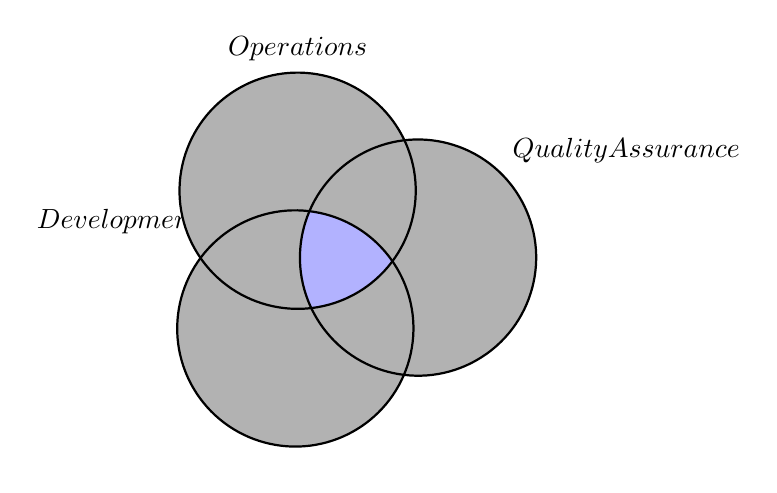
\begin{tikzpicture}[thick,
    set/.style = {circle,
        minimum size = 3cm,
        fill=black!30}]
 
% Set A
\node[set,label={135:$Development$}] (A) at (0,0) {};
 
% Set B
\node[set,label={45:$Quality Assurance$}] (B) at (1.8,0) {};
 
% Set C
\node[set,label=$Operations$] (C) at (0.9,1.5) {};

% Intersection
\begin{scope}
    \clip (0,0) circle(1.5cm);
    \clip (1.8,0) circle(1.5cm);
    \clip (0.9,1.5) circle(1.5cm);
    \fill[blue!30](0,0) circle(1.5cm);
\end{scope}
 
% Circles outline
\draw (0,0) circle(1.5cm);
\draw (1.8,0) circle(1.5cm);
\draw (0.9,1.5) circle(1.5cm);
 
\end{tikzpicture}
\caption[DevOps model]{The DevOps model\footnotemark}
\label{fig:DevOps model}
\end{figure}
\vspace{0.5cm}

\footnotetext{Impression of the reference DevOps model taken from source~\parencite[p-21]{leszko2017continuous}}



In this paper, an empirical solution for the implementation concept of \ac{CI} \ac{CD} pipeline is well presented with the preliminary work mentioned in the next chapter (see Section~\ref{section:ImplementationOutline}). The solution have been facilitated with the flexibility of the build pipeline, as well as future adaptations. For example, changes to the application source code would require no significant modifications to the build pipeline. 

\section{Software Release} \label{section:Softwareconfigurationmanagement}

\vspace{0.2cm}
\noindent \textbf{Software Configuration Management}
\vspace{0.2cm}

\noindent In proper context to the software development process, \ac{SCM} plays a quintessential part, which gives stakeholders the ability to track or control frequent changes made to the project workspace. A workspace is defined as the central location with all the files that make up the project. Developers also have the ability to configure their project workspace with a version control system (see Section~\ref{section:versioncontrol}) for better tracking of the daily changes committed to the project. A ideal example of this, are the project repositories configured with the GitHub platform. It usually consists of multiple codelines or branches which contains the progression set of source files, test suites, build scripts to define the software build and test (see Section~\ref{section:CICDpipeline}). Every modifications made to these files gets tracked with the help of revision id's. At a particular point in the development process, a snapshot of the codeline can be taken which is a configuration of the codeline and identified as versions~\parencite{berczuk2003software}. A version is particularly recognised by a prominent name or numbers. Figure \ref{fig:CodelineStructure} illustrates an typical sequence diagram of the progressive (left to right) project repository where File A and File B are the source files which goes through various modifications as the project advances. So, as denoted in circles every commits made to these files are defined by a short identifier or revisions. A particular point of the project is usually recognised with the help of version numbers, and it helps at the time of software releases. The version indicated with a prefix "v" includes several revisions in the codeline.

%----------------------------------------------------------------------------------------
\vspace{0.5cm}
\begin{figure}[H]
\centering
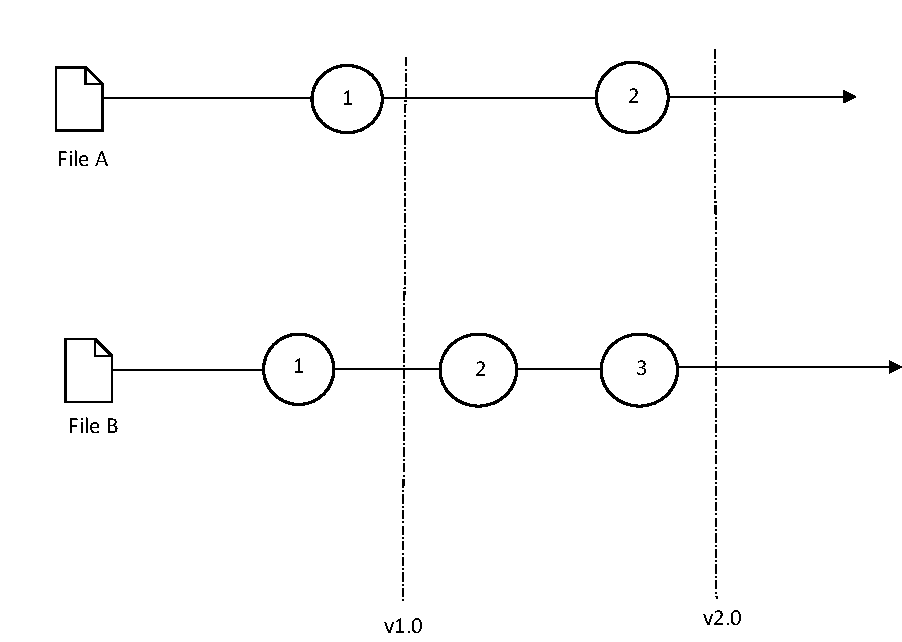
\includegraphics[scale=0.8]{figures/softwareversion.pdf}
\caption[Codeline Structure]{Codeline Structure}
\label{fig:CodelineStructure}
\end{figure}
\vspace{0.5cm}
%----------------------------------------------------------------------------------------


The practise of \ac{SCM} governs how an organization builds and releases software products, identifies and tracks changes~\parencite{berczuk2003software}. A primary motive behind \ac{SCM}, is to give developers the control and easy traceability over a project. 






%----------------------------------------------------------------------------------------
\vspace{0.2cm}
\noindent \textbf{Software Versioning}
\vspace{0.2cm}


\noindent With software versions, developers can represent a particular point of the project that is ready for release. It contains several revisions of the software component and helps to detect all the code changes, improvements and bug fixes \footnote{In GitHub platform, developers can use git tags to identify a project version.}. Versions are identified by unique version numbers. Mostly the version numbers are represented in the form of dot separated identifiers or x.y.z(where all three version components are positive integers) and tracks major changes.minor changes.patch updates committed to the software package. Release version number in the $[1.0.0; +\infty]$ range are denoted as \emph{production release} or \emph{stable release} \footnote{From \ac{SemVer} FAQ, Software packages used in production should already be 1.0.0~\parencite{preston2013semantic}, also defined as public API} while package releases with a version number in the $[0.0.0;1.0.0]$ version range are called \emph{initial development releases}~\parencite{8721084}. It is important to note that the software package version numbers are different than the product version numbers. 



%----------------------------------------------------------------------------------------
\vspace{0.2cm}
\noindent \textbf{Release Management}
\vspace{0.2cm}

\noindent     Release management process typically supervise the stages associated with software release cycle. The need for release management must be considered in the distributed software development and deployment process. The process is closely associated with \ac{SCM}. Usually, an exemplary release cycle model involves multiple stages. The release cycle begins with project developers creating independent development branches from the main branch. In a continual software development process, several changes are committed  which includes modifications to its codebase, new functionalities, bug fixes. This changes are added to the software and gets evaluated continuously before the final production release.  It runs through the entire stages of software build, testing and deployment, to ensure that the added changes does not break the existing functionalities of the software. The new flavors of the software with additional changes usually gets tracked by software version numbers. The internal stakeholders decide which features and changes are a part of the next release. The goal is to release only stable versions of the project~\parencite{russo2003toward}. A software release lifecycle identifies potential release candidate that is fit for production release.

\vspace{0.5cm}
\begin{figure}[H]
\begin{tikzpicture}[node distance=1.5cm,
    every node/.style={fill=white, font=\sffamily}, align=center]
  % Specification of nodes (position, etc.)
  \node (start)             [process] {Pre-Alpha};
  \node (onCreateBlock)     [process, below of=start]          {Alpha};
  \node (onStartBlock)      [process, below of=onCreateBlock]  {Beta};
  \node (onResumeBlock)     [process, below of=onStartBlock]   {Release Candidate};
  \node (activityRuns)      [process, below of=onResumeBlock] {Production Release};

  % Specification of lines between nodes specified above
  % with aditional nodes for description 
  \draw[->]             (start) -- (onCreateBlock);
  \draw[->]     (onCreateBlock) -- (onStartBlock);
  \draw[->]      (onStartBlock) --  (onResumeBlock);
  \draw[->]     (onResumeBlock) -- (activityRuns);

                                   
\end{tikzpicture}
\caption{Distinct approach of the software release lifecycle}\label{fig:softwarereleaselifecycleSteps}
\end{figure}
\vspace{0.5cm}

%----------------------------------------------------------------------------------------
\noindent \textbf{Pre-Alpha release}
\vspace{0.2cm}

\noindent The Pre-alpha phase of the software release cycle involves stages like requirement gathering and analysis, design and development. It involves stages prior to the actual test. Here, the software product is unstable and all the features are not complete. This is the first stage of the software development process, where the developers create the initial blueprint of the project.


%----------------------------------------------------------------------------------------
\vspace{0.5cm}
\noindent \textbf{Alpha Release}
\vspace{0.2cm}

\noindent The next phase of the software release lifecycle is the Alpha release. It involves a number of internal validation and testing techniques such as the white-box test and black-box test. Generally, the version is appended with a hyphen and a pre-release tag which immediately follows the patch version~\parencite{preston2013semantic}. For example, an alpha version of a software is tagged as x.y.z-alpha or x.y.z-a.b.c, where x, y and z denotes the major, minor, and patch identifiers and a, b and c are the pre-release identifiers. 

%----------------------------------------------------------------------------------------
\vspace{0.5cm}
\noindent \textbf{Beta Release}
\vspace{0.2cm}

\noindent Beta phase begins when the software is feature complete and all the intended functionalities are working. Subsequently, at this phase, the software is released for the first time to the intended customers (commonly referred to as beta testers) for testing. The release process is referred as \emph{Beta release}. There may be multiple beta versions in a beta cycle as the software goes through additional changes or is exposed to minor/major bugs. A beta version is also identified with the "beta" pre-release tag.


%----------------------------------------------------------------------------------------
\vspace{0.5cm}
\noindent \textbf{Release Candidate}
\vspace{0.2cm}


\noindent A \ac{RC} refers to a particular software version that is in the final stages of quality assurance. Every change is, in effect, a release candidate. If the resulting \ac{RC} is found to be error free, and it meets the customer acceptance criteria, then it is ready for production release. A release candidate is the last phase of the software release cycle prior to the actual release and can be identified with a pre-release tag "rc"~\parencite{humble2010continuous}.

%----------------------------------------------------------------------------------------
























%----------------------------------------------------------------------------------------
\section{The Embedded Linux Landscape}\label{section:embeddedlinux}

When developing an embedded operating system, there are certain criteria’s which a developer should consider.  Firstly, the target hardware is constraint of memory and space. Secondly, the microcontroller’s CPU will be much weaker in comparison to big office machines or even personal computer. So, the operating system should not only be space efficient but also deliver real time operations. The OS is notably the most crucial part of the software adaptation, which  provides abstraction from the hardware through its libraries and application programming interfaces (API)~\parencite{Reference1}. Linux OS for embedded system development is the best choice for developers due to multiple benefits. It is open-source software with lot of support for customization and most importantly the OS image size is small. For example, the Alpine Linux is only 5 MB in size. To classify broadly, there are some generic embedded OS like \emph{Android} to primarily target mobile phones hardware or \emph{OpenWrt} to target routers or modems. But mostly, companies build its own custom embedded Linux OS with a set of development tools, specifically designed for a hardware. The thesis work was also carried out on a custom Linux distribution build specially for a particular project specific hardware.

%----------------------------------------------------------------------------------------
\subsection{The Yocto Project}

As perfectly explained in the Yocto project manual~\parencite{Reference2}:
\vspace{0.5cm}


\enquote{\emph{The Yocto Project is an open source collaboration project that helps developers create custom Linux-based systems that are designed for embedded products regardless of the product’s hardware architecture.}}
\vspace{0.5cm}

It is a challenge for developers to build an embedded Linux image from scratch with no pre-build tools or software. The task of building a Linux kernel, a cross-compiler to compile the filesystem and package dependencies is extremely complex and painful. The Yocto project has simplified the process, it has many available software tools and resources to build a hardware independent custom Linux distribution image. It provides flexibility and support multiple customization depending on the project requirement. For example, the Linux distribution or the build system to support a smart home embedded device may be different to the Linux distribution meant for more complex systems. With the \ac{OE} build system as the heart of the Yocto project, all the necessary native utilities are build along with software packages by the build engine, BitBake. Bitbake processes the recipe files to define how the software packages should be build. The initial build is comparatively long, but the intermediate build stages use the \ac{SSTATE} cache mechanism that allow reuse of sstate files and this accelerates the build process. Refer to Section~\ref{section:bitbake} and Section~\ref{section:recipes} for more detailed description of BitBake and Yocto recipe files.


%----------------------------------------------------------------------------------------
\vspace{0.5cm}
\begin{figure}[H]
\begin{tikzpicture}
\begin{scope}[xshift=5.5cm]
\coordinate (O) at (0,0);
\draw[fill=gray!30] (O) circle (2.8);
\draw[fill=gray!40] (O) circle (2);
\draw[fill=blue!30] (O) circle (1.2);

\draw[decoration={text along path,reverse path,text align={align=center},text={Poky}},decorate] (0.5,0) arc (0:180:0.5);
\draw[decoration={text along path,reverse path,text align={align=center},text={OpenEmbedded build}},decorate] (1.3,0) arc (0:180:1.3);
\draw[decoration={text along path,reverse path,text align={align=center},text={The Yocto Project}},decorate] (2.1,0) arc (0:180:2.1);
%\draw[decoration={text along path,reverse path,text align={align=center},text={Hello, how are you?}},decorate] (2.9,0) arc (0:180:2.9);
\end{scope}
\draw[draw=none] (2.6,0) -- (3.0,0);
\end{tikzpicture}
\caption[The Yocto Project family]{The Yocto Project family}
\label{fig:The Yocto Project family}
\end{figure}
\vspace{0.5cm}

The Yocto Project combines multiple projects under one umbrella. The \ac{OE} project is the most prominent one. It is the build framework for developing the custom Linux distribution.The \ac{OE} build system includes \emph{BitBake}, the \emph{\ac{OE} core} and the reference distribution \emph{Poky}~\parencite{Reference1}.
%----------------------------------------------------------------------------------------

\subsection{Poky}

OpenedHand, an embedded Linux startup company developed Poky Linux, the Linux distribution build with \ac{OE} for mobile device~\parencite{Reference1}. Independent of the target hardware, poky offers cross-compilation environment with the help of BitBake , \ac{OE}-core layers, and set of metadata layers. It simplifies the process of configuring the Linux image for the target embedded device by providing a framework of all the necessary components by combining multiple open-source projects for pre-configured embedded Linux OS stacks, and adapt or modify the original framework to bootstrap the actual system development. Poky can either be installed from git or from unpacking the tarball downloaded from the Yocto project website. However, the former is preferred as you get regular code updates automatically which can be applied easily to the codebase. At the starting development phase of the project, the reference distribution Poky git repository is cloned, creating a copy in the local machine which creates the Source Directory where the Yocto development work takes place. The directory tree structure is depicted in Figure \ref{fig:Source Directory layout}. The directories are outlined with proper icon and their names are italicized to distinguish them from filenames.




%----------------------------------------------------------------------------------------
\vspace{0.5cm}
\begin{figure}[H]
\par\noindent
  \centering 
\begin{forest}
  pic dir tree,
  where level=0{}{% folder icons by default; override using file for file icons
    directory,
  },
  [SOURCE DIRECTORY
    [\textit{Yocto}
    [\textit{Poky}
        [\textit{BitBake}]
        [\textit{Meta- layers}]
        [\textit{Documentation}]
        [LICENSE, file]
        [README, file]
    ]
    ]
  ]
\end{forest}
\caption[The Source Directory layout]{The Source Directory tree contains BitBake, documentation, metadata layers which are compatible to the Yocto project and its creation is the first step towards developing the custom Linux distribution}\label{fig:Source Directory layout}
\end{figure}
\vspace{0.5cm}



The \emph{Source Directory} (also termed as the poky directory)includes all the base and custom metadata layers, recipes, and other essential files. As illustrated in Figure~\ref{fig:Poky: the reference distribution of Yocto project}, poky works cohesively combining the given set of base and custom components to build a complete customizable Linux OS stack~\parencite{salvador2014embedded}. With Poky, a custom and intuitive Linux distribution can be build to support different hardware platforms or machine configurations.
%----------------------------------------------------------------------------------------
\vspace{0.5cm}
\begin{figure}[H]
\centering
\begin{tikzpicture}[block/.style={regular polygon,regular polygon sides=4,
    inner xsep=2em,align=left,text width=5em,draw},font=\sffamily,thick,
    box/.style={draw,align=left,inner sep=2em},>=stealth
  ]
 \begin{scope}[local bounding box=blocks]
  \node[block,fill=gray!20] (B1) {OpenEmbedded-Core};
  \path let \p1=($(B1.east)-(B1.west)$) in 
  node[right=4em of B1,block,fill=gray!20] (B2) {meta-yocto (Yocto specific metadata)};
 \end{scope} 
 \path let \p1=($(blocks.east)-(blocks.west)$) in
  [nodes={minimum width=\x1},node distance=2em]
  node[box,fill=gray!20,above=of blocks] (A) {Bitbake}
  node[box,fill=gray!20,below=of blocks] (C) {meta-yocto-bsp (Yocto specific BSP)};
 \node[draw=gray,thin,fit=(A)(C),dashed,rounded corners=0.8em,inner sep=0.8em,
    label=right:Poky Build]{};
\end{tikzpicture}
\caption[Poky: the reference distribution of Yocto project]{Poky: the reference distribution of Yocto project\footnotemark}
\label{fig:Poky: the reference distribution of Yocto project}
\end{figure}
\vspace{0.5cm}
\footnotetext{The reference figure has been depicted from source~\parencite[p-8]{salvador2014embedded}}
%---------------------------------------------------------------------------------------
\subsection{BitBake} \label{section:bitbake}
The task executor, BitBake is the build engine at the core of \ac{OE} build system and the Poky reference distribution. During the build process, BitBake process the metadata, configuration files, class files, recipe files. BitBake, evolved from Portage, the build and package management of Gentoo Linux uses same metadata syntax as Portage build scripts. It also have features like the inheritance mechanism which is supported by classes, appending recipes, and global configuration files~\parencite{Reference1}. The first step in a cross-platform BitBake build process is to create a cross-compile toolchain for the target platform, which then build the other required elements~\parencite{veromannembedded}.


The result produced after a successful build process is the binary output called image. It is stored in the Build Directory of the \ac{OE} build environment. The \emph{Build Directory} stores the output generated by the BitBake build process and it is configured when the \ac{OE} build environment is set up (See the setup script in listing~\ref{lst:listing-sourcebuild}). Running the source command in a shell environment creates the Build Directory, and it should be set up before any BitBake process. The Build Directory name defaults to \texttt{build/}, if the user have not set up and the \texttt{TOPDIR} global variable refers to the Build Directory.

\vspace{0.5cm}
\lstset{style=mystyle}
\lstinputlisting[caption=The OpenEmbedded Build Environment setup script, captionpos=b,   basicstyle=\footnotesize, frame=lines, numbers=left, label={lst:listing-sourcebuild}, language=bash]{code/source.sh}
\vspace{0.5cm}

Figure \ref{fig:yoctobuilddir} illustrates the contents of the Build Directory. It includes the \texttt{cache} directory which stores machine specific cache files, output files like the target filesystem images, license files are stored inside the \texttt{deploy} directory under \texttt{temp} folder. All the user configurations files are stored under the \texttt{conf} directory. More details on the user configuration files will be discussed in the next section.

\vspace{0.5cm}
\begin{figure}[H]
\centering{{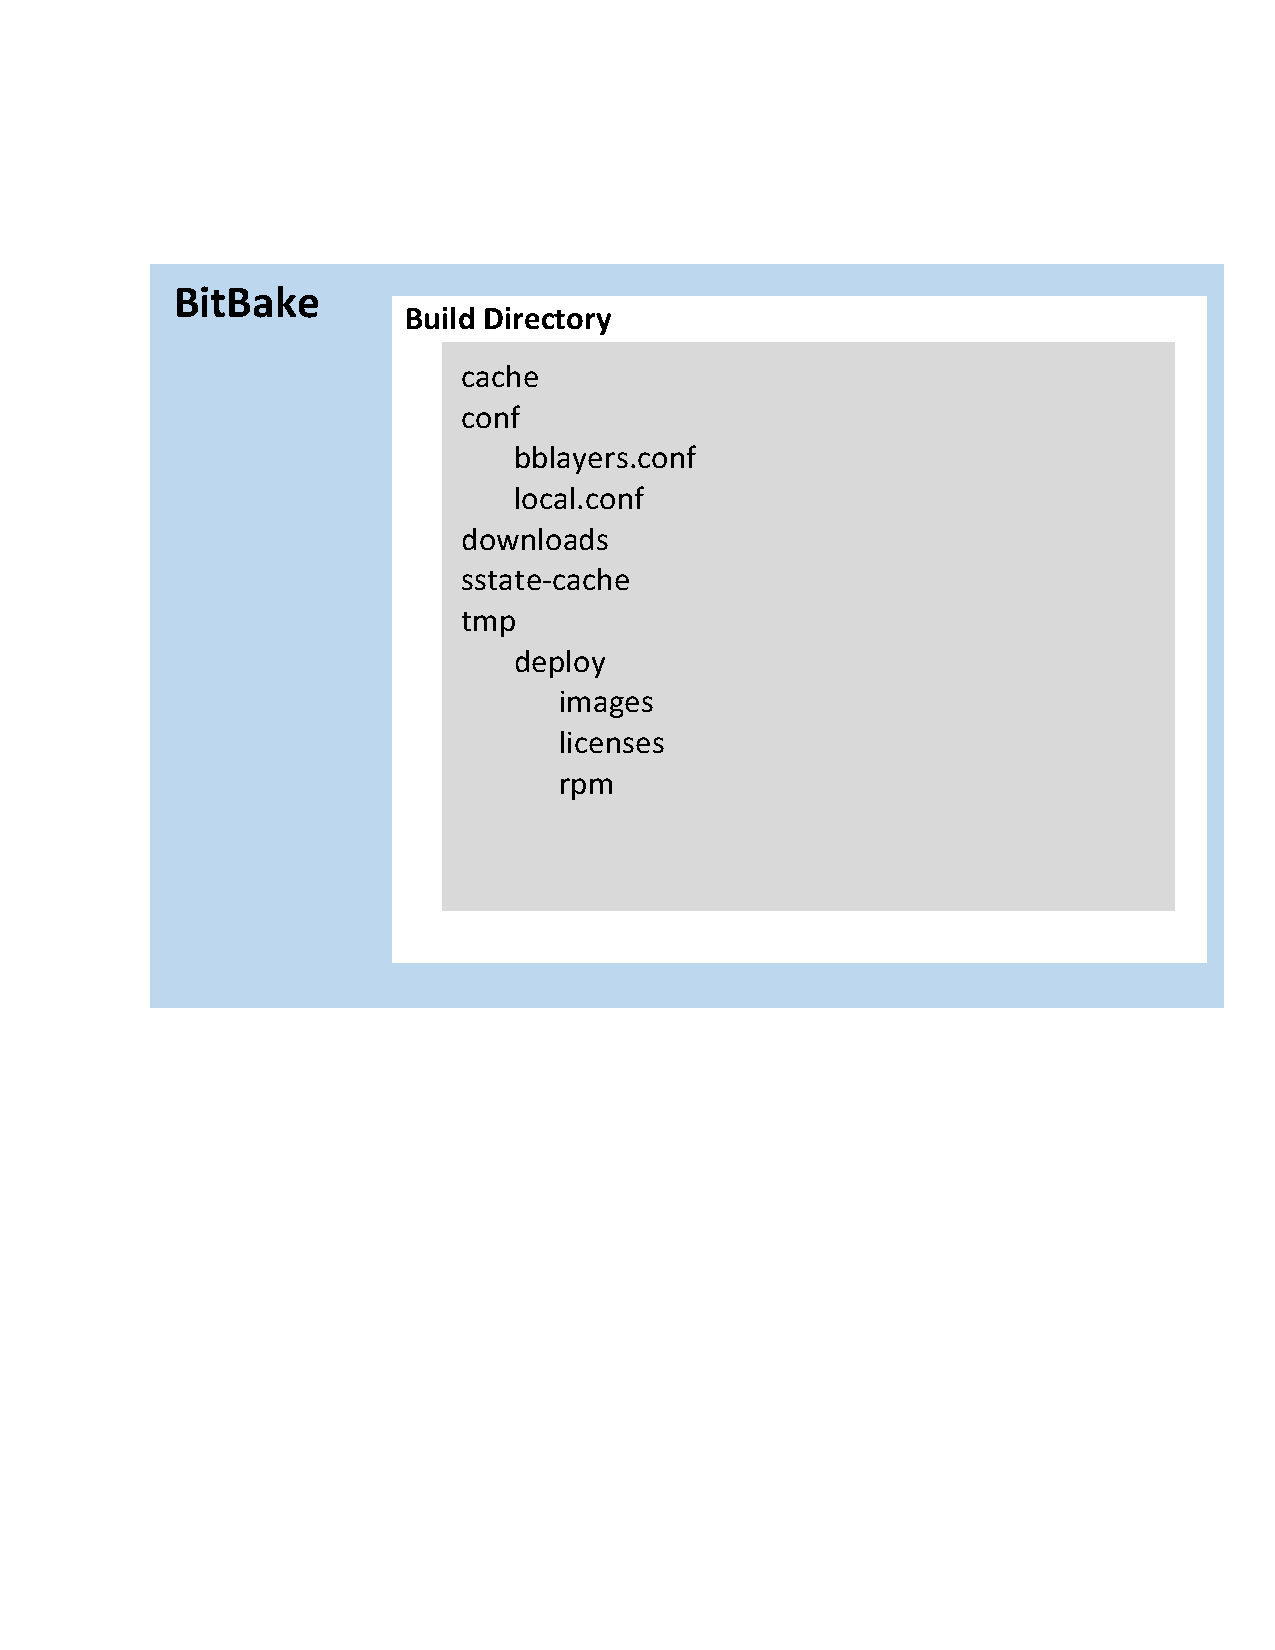
\includegraphics[width=0.7\textwidth]{figures/BitBake build directory.pdf} }}%
\caption{The Yocto Build Directory}
\label{fig:yoctobuilddir}
\end{figure}
\vspace{0.5cm}

%---------------------------------------------------------------------------------------
\subsection{Configuring the Build Directory}

The build directory contains two important user configuration files:

\begin{itemize}
 
\item{bblayers.conf} – This file contains the list of all the metadata layers which are needed by BitBake to run during the build. The file is named as \texttt{bblayers.conf} and is stored inside the \texttt{conf} directory within the Build Directory. The listing~\ref{lst:listing-bblayers} below illustrates a sample bblayers.conf file. Here, \texttt{YOCTO\_LAYERS} includes all the base layers predefined by the Yocto Project and essential to run the build. \texttt{EXTRA\_LAYERS} and \texttt{BOSCH\_TT\_LAYERS\_PLATFORM} denotes all the custom, user-defined layers specific to the project. 

\vspace{0.5cm}
\lstset{style=mystyle}
\lstinputlisting[caption=A bblayers.conf list all the conventional default Yocto layers and additional Bosch layers for building a custom Yocto image, captionpos=b,   basicstyle=\footnotesize, stepnumber=1, frame=lines, numbers=left, label={lst:listing-bblayers}, language=Python]{code/bblayers.conf}
\vspace{0.5cm}

Any variable set by using the "=" overrides the same variable value set elsewhere, also known as hard assignment. "?=" is the soft assignment which means the variable will not be set if defined somewhere else in the environment.


\item{local.conf} – The local configuration or the \texttt{local.conf} file within the build directory or precisely inside the \texttt{conf} directory stores project specific information and  parameters like selection of the target machine via \texttt{MACHINE} parameter, packages needed in the final image, types of packages (debian, rpm, ipk) and distribution to use via \texttt{DISTRO} parameters~\parencite{swain2015design}. For example, consider the following listing~\ref{lst:listing-localconf} below where a minimal local.conf file is configured for the \texttt{poky-boschtt-systemd} distribution for the machine type \texttt{commodul}. \texttt{MIRRORS} and \texttt{PREMIRRORS} parameter variables for recipe source \ac{URL} redirection can also be set in the local configuration file.

\vspace{0.5cm}
\lstset{style=mystyle}
\lstinputlisting[caption=Local user settings according to the target requirements of the custom Yocto image are set in the local.conf file, captionpos=b,   basicstyle=\footnotesize, stepnumber=1, frame=lines, numbers=left, label={lst:listing-localconf}, language=Python]{code/local.conf}

\vspace{0.5cm}
\end{itemize}

One can also make use of Hob, a graphical user interface for BitBake by the Yocto project to set or modify the \texttt{local.conf} and \texttt{bblayers.conf} conveniently without any physical intervention to the actual file. It enables the user to select the base image type or packages needed for the target image from the \ac{GUI} itself. Hob will automatically make suitable changes in these files~\parencite{swain2015design}. 
%----------------------------------------------------------------------------------------
\subsection{Recipes and Class} \label{section:recipes}

Among other metadata files, recipes and class files are most used in the build process. All the software package information are stored in the recipe file. Creating custom recipes for  target hardware is always preferable since it could be tailored to suit the exact target requirements~\parencite{swain2015design}. One can recognize a recipe file with the \texttt{.bb} extension. BitBake uses recipes to define how the software packages are build. Recipes contain information about the required software packages, dependencies, instructions to compile the source files and package the compiled output~\parencite{veromannembedded}. While writing a recipe file for a particular software package, there are certain conventions one needs to follow. For example, the filename are usually in the form of <\texttt{softwarepackage\_version.bb}>, where softwarepackage denotes the package name. An underscore divides the version string and the package name. Typical examples of a recipe filename are <\texttt{restapi\_v3.7.0.bb}> or <\texttt{comd\_v3.7.0.bb}>. BitBake interprets the \texttt{softwarepackage} or \texttt{version} correctly to its predefined variables \texttt{PN}, \texttt{PV} used in the OpenEmbedded build system. A mismatch in the recipe filename or the version will lead to incomplete build process and can result to error in installing the particular software package. In contrast to configuration files, the variable assignments made within the recipe are local to the recipe only~\parencite{ Reference1}. 



One feature offered by BitBake is sharing the common functionalities between recipes via BitBake \texttt{classes}, identified by \texttt{.bbclass} suffix. The classes provide base methods and are used to define the behaviour of the build system. The recipes and the classes contains code written in shell script or python code~\parencite{salvador2014embedded}. The class file (\texttt{.bbclass}) includes the task definitions written in BitBake style functions that are inherited by recipes but cannot be directly executed by BitBake~\parencite{violanteembedded}. Basically, the task definitions are executable set of instructions provided by BitBake. BitBake tasks have always a standard \texttt{do\_} prefix in the name. To use the functionality of a class, the recipe uses the \texttt{inherit} directive. The listing \ref{lst:listing-recipeurl} uses the BitBake class inheritance feature, to inherit the \texttt{packageclass} class functionality into its recipe. Another BitBake feature is the \texttt{append} files, commonly used by layers to build on top of other layers to tweak variable settings in the recipes contained in those layers for special requirements~\parencite{Reference1}.

%----------------------------------------------------------------------------------------
\subsection{Metadata layer and metadata files}

Layers are the repositories inside the build environment. It functions like containers to group and organize recipes, classes, configuration files, and other metadata into logical entities~\parencite{Reference1}. Figure \ref{fig:Meta layer architecture} illustrates the meta layer architecture in the \ac{OE} build system. A build system holds multiple layers to store different software packages like \ac{BSP} layer for the hardware, \ac{GUI} layer, Distribution layer required for the OS configuration, application layer for additional software package needed for the image. It is a recommended practice to create own layers for additional software packages rather than having only one single layer to define all the image components. For example, the software packages specific to the project requirement are mostly isolated into one single layer. The advantage of layer isolation is to foster the future modifications needed according to project requirements. On top of it, layers define its own classes and recipes.

\vspace{0.5cm}
\begin{figure}[H]
\centering
\tikzset{
  planet/.append style={regular polygon, regular polygon sides=6},
  satellite/.append style={regular polygon, regular polygon sides=6},
  every picture/.append style={rotate=30},
  connection planet satellite/.style={
    bend right/.style=,
    every edge/.style={fill=\col},
    to path={
      \pgfextra
        \path[draw=none, fill=none] (\tikztostart) 
          -- coordinate[at start] (@start@) coordinate[at end] (@target@) (\tikztotarget);
      \endpgfextra
      \ifnum\xi<8 % to disable the last arrow
        ($(@start@)!.6cm!90:(@target@)$) -- ($(@target@)!.25cm!-90:(@start@)$)
          -- ($(@target@)!.25cm!90:(@start@)$) -- ($(@start@)!.6cm!-90:(@target@)$)
          -- cycle
      \fi}}}
\smartdiagram[connected constellation diagram]{
  Metadata Layer Structure,
  Application Layer,
  GUI Layer,
  Distribution Layer,
  \ac{BSP} Layer,
  Poky Layer,
  OE Core Layer}
\caption[Meta layer architecture]{Layers group metadata into logical entities. Layers commonly build on and extend each other~\parencite{Reference1} }
\label{fig:Meta layer architecture}
\end{figure}
\vspace{0.5cm}


The recipe are mostly grouped by categories which stores a collection of recipes that defines the same category. For example, \texttt{recipes-bosch} of \texttt{meta-software} would contain all the recipes that build the software components implemented and licensed by Bosch group and are required for the creation of the root filesystem image. Within a single category, there are subdirectories to define individual software packages that contains the recipe files, configurations. By convention, the name of the top-level directory of a layer is mostly prepended with a prefix \texttt{meta} followed by a hyphen and the layer name. To understand the directory structure better, refer to the following Figure \ref{fig:Layer layout} (directories are outlined with proper icon and their names are italicized to distinguish them from filename) where the \texttt{meta-software} layer directory tree includes the bosch recipes and client recipes and its subdirectory for software packages. The \texttt{conf} subdirectory is essential in every layer which contains the layer configuration file \texttt{layer.conf} which identifies the file structure as a layer, contents of the layer and instructions about how the build system should use it~\parencite{Reference2}. Each layer has its own \texttt{layer.conf}. It is important to note that a package subdirectory contains recipes to build different versions of that particular package~\parencite{Reference1}.

\vspace{0.5cm}
\begin{figure}[H]
  \centering
\begin{forest}
  pic dir tree,
  where level=0{}{% folder icons by default; override using file for file icons
    directory,
  },
  [meta-software
    [\textit{classes}
        [aclass.bbclass, file]
        [bclass.bbclass, file]
    ]
    [\textit{conf}
        [layer.conf, file]
    ]
    [\textit{machine}
        [amachine.conf, file]
    ]
    [\textit{distro}
      [distro.conf, file]
    ]
    [\textit{recipes-bosch}
        [package 1
            [package1\_version.bb, file]
        ]
        [package 2
            [package2\_version.bb, file]
        ]
    ]
    [\textit{recipes-client}
      [package 1
            [package1\_version.bb, file]
        ]
        [package 2
            [package2\_version.bb, file]      
      ]
    ]
  ]
\end{forest}
\caption[Structure of the metadata layer directory]{A basic layout of the metadata layer where recipes files for software packages, layer configuration file and class files are defined}\label{fig:Layer layout}
\end{figure}
\vspace{0.5cm}

The \ac{OE} build environment contains few sets of predefined base layers and special custom layers typically implemented according to the machine requirement. The OE Core is the main base for the layer architecture. It is the main Yocto Project layer maintained by the \ac{OE} community and by the Yocto project~\parencite{violanteembedded}. It contains the recipes for core packages like the bootloaders, networking, kernel and provides base classes to build the software packages, create filesystem images, and extend the BitBake functionality~\parencite{Reference1}. Table 2.2 outlines the general and special metadata layers that are Yocto and \ac{OE} compatible and highlight its importance.
%----------------------------------------------------------------------------------------

\vspace{0.5cm}
\begin{table}[H]
\caption{Metadata Layer Layout}
\renewcommand{\arraystretch}{1.5} 
\begin{tabularx}{\textwidth}{@{}lXSS@{}}
\toprule
\multicolumn{1}{l}{Layer}&\multicolumn{1}{l}{Description}\\
\midrule
Application Layer& Custom layers to build software packages for the target image. It is specific to the project requirement and product use case.\\
\ac{GUI} Layer& Layer to define the \ac{GUI} environment and user interface.\\
Distribution Layer &  Specifies the policy configurations for the images of a distribution, OS configurations for user accounts, system startup~\parencite{Reference1}. \\
BSP Layer & Special layer to define specific target machine and hardware configurations and also contains information about the kernel.\\
Poky Layer& Base layer for the poky reference distribution.\\
\ac{OE} Core Layer& The \ac{OE} Core layer is the core metadata of the poky build system. It includes all the necessary set of recipes needed to build a Linux OS stack.\\
\bottomrule
\end{tabularx}
\end{table}
\vspace{0.5cm}
The poky distribution includes the \ac{OE} build system as well as the three metadata layers \ac{OE} Core (meta), Yocto distribution (meta-yocto), and Yocto BSP (meta-yocto-bsp) and are automatically added at the creation of the build environment~\parencite{Reference1}. 


































%----------------------------------------------------------------------------------------
\subsection{Building Software Packages} \label{section:softwarepackageinrecipes}

In general, BitBake can execute tasks which includes shell functions written in shell scripts and BitBake style python functions. Existing class files also have predefined tasks that can be called into recipes and classes. One special example will be the \emph{base.bbclass} which contains a set of common functionalities and is automatically included in all recipe and class files~\parencite{team2006openembedded}. One can also make use of the regular python functions inside a recipe file or class file. This section will provide a detailed overview of how BitBake executes task to build the application package with the help of recipe files. A portion of the research work also conducted by leveraging the power of the BitBake task or regular python functions. The BitBake tasks are only recognised by the recipe files (.bb) or class files (.bbclass) which are inherited from the recipe files. 

\begin{itemize}
 
\item \keyword{Fetch} - The first step of the obtaining the software package into the build environment is defining a source file path or source address. Typically, it is written within the recipe (.bb) file, usually defined with the variable name "SRC\_URI". The source can be local or remote file servers or revision control systems like Git, Subversion, and others. Remote \ac{URL} sources such as download sites or repositories are commonly supplemented with trailing patches number and auxiliary files that are stored on a local filesystem~\parencite{Reference1}. This can however be defined with other custom variable names as well. BitBake offers several download fetcher protocols like \ac{FTP} and \ac{HTTP}. 

BitBake provides the necessary tools for retrieving the source code packages from many sources. The recipe file configured in the thesis work (See Section~\ref{section:implementationconcept}) had implementations to fetch the source code of the released version of the software package from \ac{HTTP} or \ac{HTTPS} source with the help of wget fetcher and Bosch development source control management system like GIT, with the help of GIT fetcher. Fetching the source from remote is very flexible and easily adaptable as well. An example recipe file in the listing \ref{lst:listing-recipeurl} below contains the source \ac{URL} addresses of a software package.

\vspace{0.5cm}
\lstset{style=mystyle}
\lstinputlisting[caption=A sample recipe file that provides the software package source, captionpos=b,   basicstyle=\footnotesize, stepnumber=1, frame=lines, numbers=left, label={lst:listing-recipeurl}, language=Python]{code/recipeurl.bb}
\vspace{0.5cm}

\item \keyword{Download and Unpack} - Followed by fetching the software package source code, it is downloaded via the download( ) method and unpacked into a specified directory inside the \emph{Work Directory} also referred by \texttt{WORKDIR} variable . The Work Directory stores extracted source package and files. Commonly, the source code is wrapped into compressed tar archives. Depending on the requirement, different compression formats can also be used.  The Work Directory also holds the log files and run or installation files which are generated at the time when BitBake executes recipe file.  BitBake uses multiple search methods to get the source package downloaded when it fails to access the original \ac{URL} mentioned in the recipe file. For example, fetching via \texttt{MIRRORS} and \texttt{PREMIRRORS} path variable defined in the recipe itself or \texttt{conf/local.conf}. One very important concept in the process of download and unpacking, is the checksum verification for file integrity. BitBake fetcher also verifies the checksum or hash values for archive downloads.  A \texttt{.done} stamp is also placed after the download is complete and checksum is verified, to avoid downloading the same source again during subsequent builds. The extracted source within the WORKDIR is usually downloaded and unpacked in the form <packagename>-<version>.

\item \keyword{Patch and Install} - Modifications to the source code is done via patching. There are various reasons why source code requires patching: adding functionalities, applying bug and security fixes, providing configuration information, or adjustments for cross-compiling~\parencite{Reference1}. Install step usually means copying source files, configuration, or binaries to user-defined target directories. It is done via the shell \texttt{install} command. The install utility can also set file ownership and permissions while copying the files~\parencite{Reference1}.
\end{itemize}


%----------------------------------------------------------------------------------------
\subsection{Images} 

The images  are  essentially configured  packages that generate a filesystem~\parencite{veromannembedded}. The final aim of developing a custom Linux distribution and the build process is the target image. The bootable image can then be flashed on the hardware. Final images are placed inside the image folder within the deploy  directory.  One can also make use of reference pre-made image that Poky distribution offers and implement custom images from it.  This work also implemented a custom Linux distribution using the reference \texttt{core-image-minimal} image which Poky offers.

One can also use other Poky distribution reference images. The “core-image-full-cmdline” for console-only image,with full functionality of featured Linux system. or \texttt{core-image-x11} image for a basic \ac{GUI} experience~\parencite{veromannembedded}. 



%----------------------------------------------------------------------------------------
\section{Integration and  Delivery at the Product level}\label{section:SoftwareIntegrationDeliveryProductLevel}

As the previous sections introduces the general picture of embedded Linux systems with the Yocto project and the basics of software integration and delivery, this section is more focused towards identification of the Yocto level integration. With this section, the first step towards understanding the subject matter of the work is achieved. It gathers and presents a implementation background of how integration of software packages and delivery of yocto image and other components work at a product level. It serves as a baseline to quantify the implementation approach (see Section~\ref{section:implementationconcept}) presented to fulfil the following aim of the thesis work. 

\vspace{0.2cm}
\begin{itemize}
\item \emph{Will BitBake solve the purpose of integrating the in-focus deliverable into the Yocto delivery package ?} 
\end{itemize}
\vspace{0.2cm}


\noindent The end goal of the Yocto project implementation for the target embedded product is to deliver the project deliverables packaged into a single delivery location or an artifactory. Among other deliverables, the delivery package includes the Linux \ac{OS} image which is ready to be flashed into the embedded device, integrated with all the required software packages and dependencies. As a part  of the base metadata layers, the default packages which are defined in the recipe provides a basic Linux OS distribution. Hence, additional packages that are integrated into the root filesystem (also referred as \emph{rootfs}) image are written as a part of custom metadata layers. 


Ultimately, at the end of the build process, the product image should have a ready-to-use rootfs for the target hardware product. It can be made up of one or more filesystems and may include other artifacts to be available during its generation, such as the Linux kernel, device tree, and bootloader binaries~\parencite{salvador2014embedded}. In order to facilitate the process of software integration at ease within the department, the software components included in the Yocto image are continuously integrated via an automated integration pipeline or precisely, the Jenkins pipeline. This evades the manual effort of setting up a physical build host system. Figure \ref{fig:softwareIntegrationAtProduct} presents a top-level view of the automated process of the Yocto level integration and delivery with the help of a continuous build pipeline.




%----------------------------------------------------------------------------------------
\vspace{0.5cm}
\begin{figure}[H]
\begin{tikzpicture}[node distance=1.5cm,
    every node/.style={fill=white, font=\sffamily}, align=center]
  % Specification of nodes (position, etc.)
\node (start)             [buildrepo, drop shadow]              {Project Build Repository\\(Metadata Layers + \\Jenkinsfile + \\Build Script)};
\node (ContinuousPipeline)      [middle, below of=start, drop shadow, yshift=-1.9cm]   {Continuous Pipeline\\ Build};
\node (Integrate)     [middle, below of=ContinuousPipeline, drop shadow, yshift=-0.8cm]   {Integrate\\Metadata\\Layer Repositories};
\node (Artifactory)      [middle, below of=Integrate, drop shadow, yshift=-2.0cm]
                                                      {Release Artifactory\\Delivery Package\\(Product Image + \\Release Notes + \\License Files)};
\node(success) [below of=Artifactory, yshift=-1cm] {success}; 

\draw[->]     (start) -- node[text width=4cm]
                                   {Stage: Software Integration}(ContinuousPipeline);
\draw[->]      (ContinuousPipeline) --  (Integrate);
\draw[->]     (Integrate) -- node[text width=4cm]
                                   {Stage: Product Delivery}(Artifactory);
\draw[->]     (Artifactory) -- (success);
                                   
\end{tikzpicture}
\caption[Software Integration at a product level]{Unified process of software integration into the product image. To accelerate the process, a \ac{CI} \ac{CD} pipeline is configured which automates the process of integration and delivery}\label{fig:softwareIntegrationAtProduct}
\end{figure}
\vspace{0.5cm}


At the beginning, the build repository of the project is implemented and hosted via the Git version control platform, which includes the necessary manifest. A \emph{manifest} contains source information about metadata layers or in simple terms, the information about the individual layer repositories which contains all the configurations, recipes, and classes. The layer repositories are easily distinguishable as their names usually prepend with \texttt{meta}. As previously stated in the layer section, this project build environment also contains base layers which are essential to build a Linux OS stack as well as special layers designed for additional software components which are project specific. The high-level view of how the software components get integrated into the product image during the build process is via recipes and layers. These recipes are files that hold information about the source \ac{URL} of the software package and how to fetch a particular software within the build. Besides, the build process is also influenced by software package versions in the recipe file. This is a general practice, as the version specified in the recipe file will download and build the exact software package. Yocto recipes follow a standard naming convention for adding versions with the package name (see section~\ref{section:recipes}). The process of how software package are installed in the Yocto build system is explained in depth in Section~\ref{section:softwarepackageinrecipes}. Additionally, versioning helps the product release cycle as BitBake builds a particular software package versions for the filesystem image. It helps tracking the deliverables much easier and also the entire lifecycle of a product gets improved. The continuous pipeline implemented in the project take care of the Yocto build process, integrating all the software components and creating a rootfs image. The image and all other components are then packed into a delivery package and then deployed to a release artifactory like JFrog.

A \emph{Release artifactory} typically stores the product artifacts inside a delivery package or folder, and with a integration pipeline in place, the software packages are continuously integrated and included into the final rootfs of the product image. With continuous integration, software accuracy can be reached at better level and the overall delivery time of the product image becomes faster. After the final delivery stage, when the image is mounted on the target hardware, the developer have the possibility to check the software versions via \ac{GUI} or \ac{CLI} of the custom Linux \ac{OS}, which is indeed helpful. The implementation work also experiments with the current delivery package and find ways to add the missing deliverable (test reports of the implemented software packages) into it.



















%----------------------------------------------------------------------------------------
\section{Summary}



\clearpage\null\thispagestyle{empty}

